\section{approach}
\label{sec:approach}
This section presents our RTRIP approach. At first, it sketches UML SM concepts. The outline and the detail of the approach are presented afterward.
\subsection{Background}
UML SM is widely used as a means to modeling the behavior of a component in complex, reactive systems. A SM has a number of possible states and well-defined conditional transitions between states. A state is either an atomic state, a hierarchical state that is composed of sub-states and has at most one active sub-state at a certain time, or a concurrent state which could have several active sub-states at the same time. Only one of the inner states of the SM can be active at a time. A state can have associated actions such as entry/exit/doActivity executed in the running of the SM. The active state of the machine can be changed to another state triggered by external or internal events. An action can also be activated by the trigger in transitioning from one state to another one.  

Our RTRIP approach is based on the double-dispatch pattern presented in \cite{spinke_object-oriented_2013} for mapping from UML SM to UML classes and traceability-mapping management in RTRIP. Figure \ref{fig:outline} shows the outline of our RTRIP approach consisting of a forward and a backward process. In the forward process, a SM is transformed into UML classes which contain attributes, operations and a block of text as method body associated with each implemented operation. The transformation uses several patterns which will be presented later. A tracing information table is created in the transformation to be used in the backward direction of the RTRIP. The UML classes are then used as the input of a classical code generator to create source code. This generation step also puts mapping from UML classes to object-oriented source code in a second mapping table.

In the backward (reverse) direction, when the source code is modified, a verification process checks whether the modified code conforms to the SM semantics (see Section C for the detail of the verification). The backward transformation takes as input the tracing tables, the created UML classes and the SM to update these models sequentially. While the forward process can generate code from hierarchical and concurrent SMs, the backward one only works for hierarchical machines excluding some pseudo-states which are \ti{history}, \ti{join}, \ti{fork}, \ti{choice} and \ti{junction}. These features are in future work.

\begin{figure}
\centering
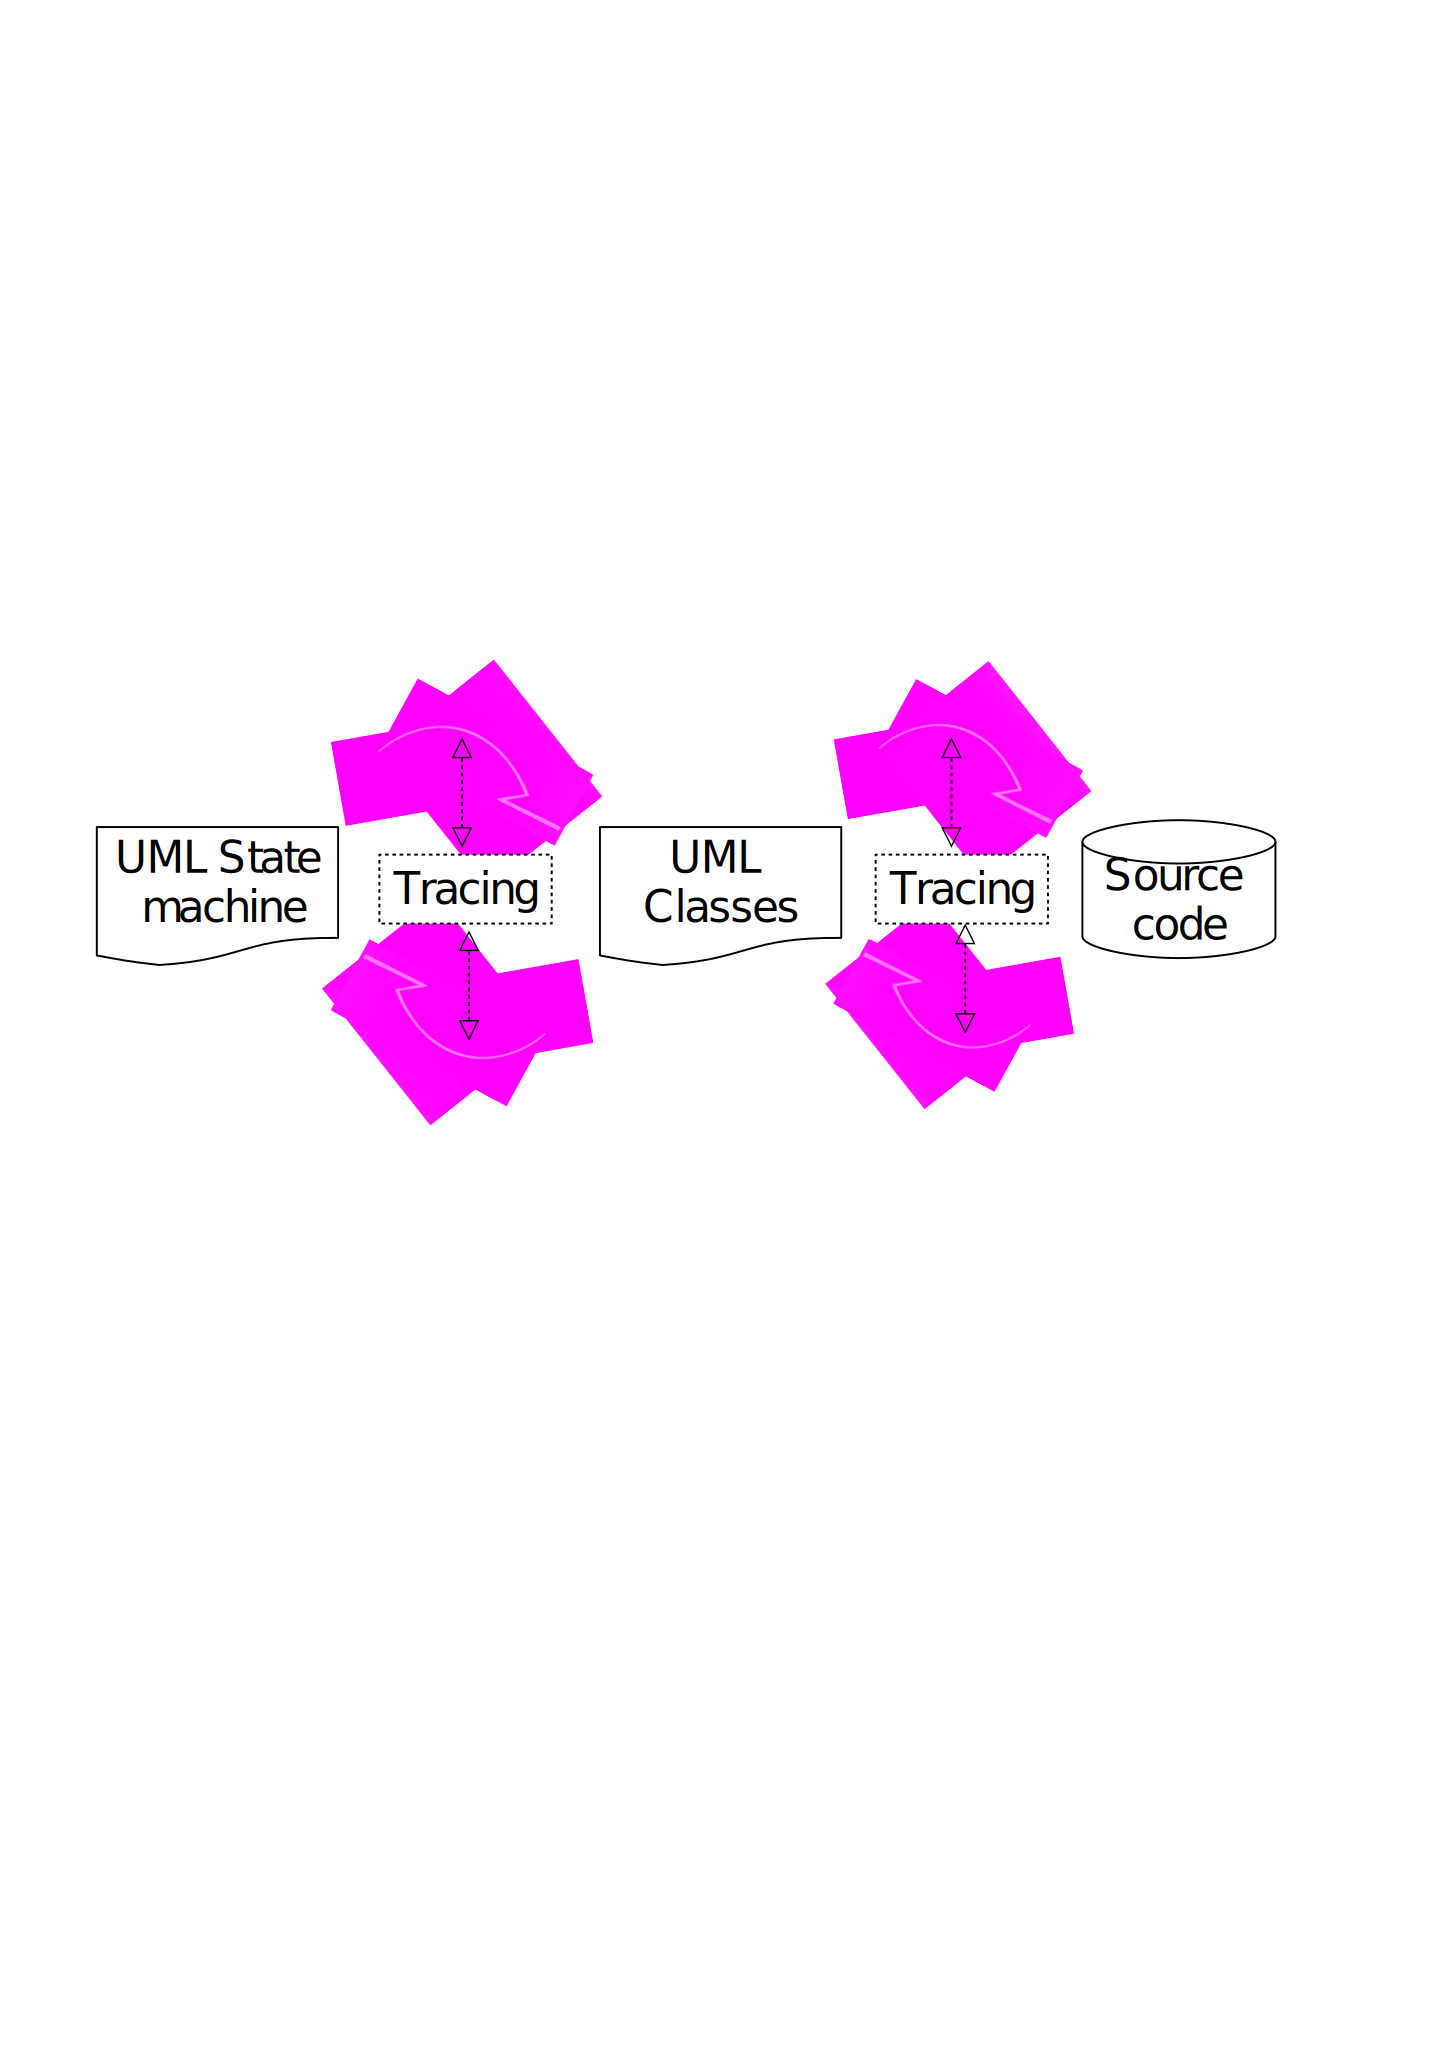
\includegraphics[clip, trim=0.5cm 10.4cm 0.5cm 7.0cm, width=0.45\textwidth]{figures/rte}
\caption{Outline of State machine and code RTE} 
\label{fig:outline}
\end{figure}

\subsection{From UML state machine to UML classes}
This section describes the forward process. The latter consists of transforming UML SM elements (see \ref{subsec:states}, \ref{subsec:events}, \ref{subsec:transitions}) into the intermediate model, storing tracing information (see \ref{subsec:trace}) and code generation (see \ref{subsec:codegen}) from the intermediate model.

\subsubsection{Transformation of states}
\label{subsec:states}
This sub-section describes the transformation of states to the intermediate model. 

This paper considers a component as a UML class called context class. Each state of the SM is transformed into a UML class in an intermediate model instead of directly generating object-oriented code as in \cite{Niaz2005}. Each UML class representing a state inherits from a base state class in the intermediate model. The base state class defines a reference to the context class, a process event operation for each event in the SM and other operations as the double-dispatch (DD) approach in \cite{spinke_object-oriented_2013}. A state class \ti{s} also has an attribute referring to the state class associated with the composite state containing \ti{s}. A composite state class has an attribute pointing to a state instance indicating the active sub-state of the composite state and a \ti{dispatchEvent} operation (see \ref{subsec:codegen}) dispatching incoming events to the appropriate active state. An example of this transformation in shown in Figure \ref{fig:hierarchical-class}. The \ti{ParentState} and \ti{SubState} are vertexes of the SM describing the \ti{Client} component, for instance. The \ti{State} and \ti{CompositeState} classes are library classes. The \ti{ParentState} inherits from the \ti{CompositeState} class since it is a hierarchical state.

\begin{figure}
\centering
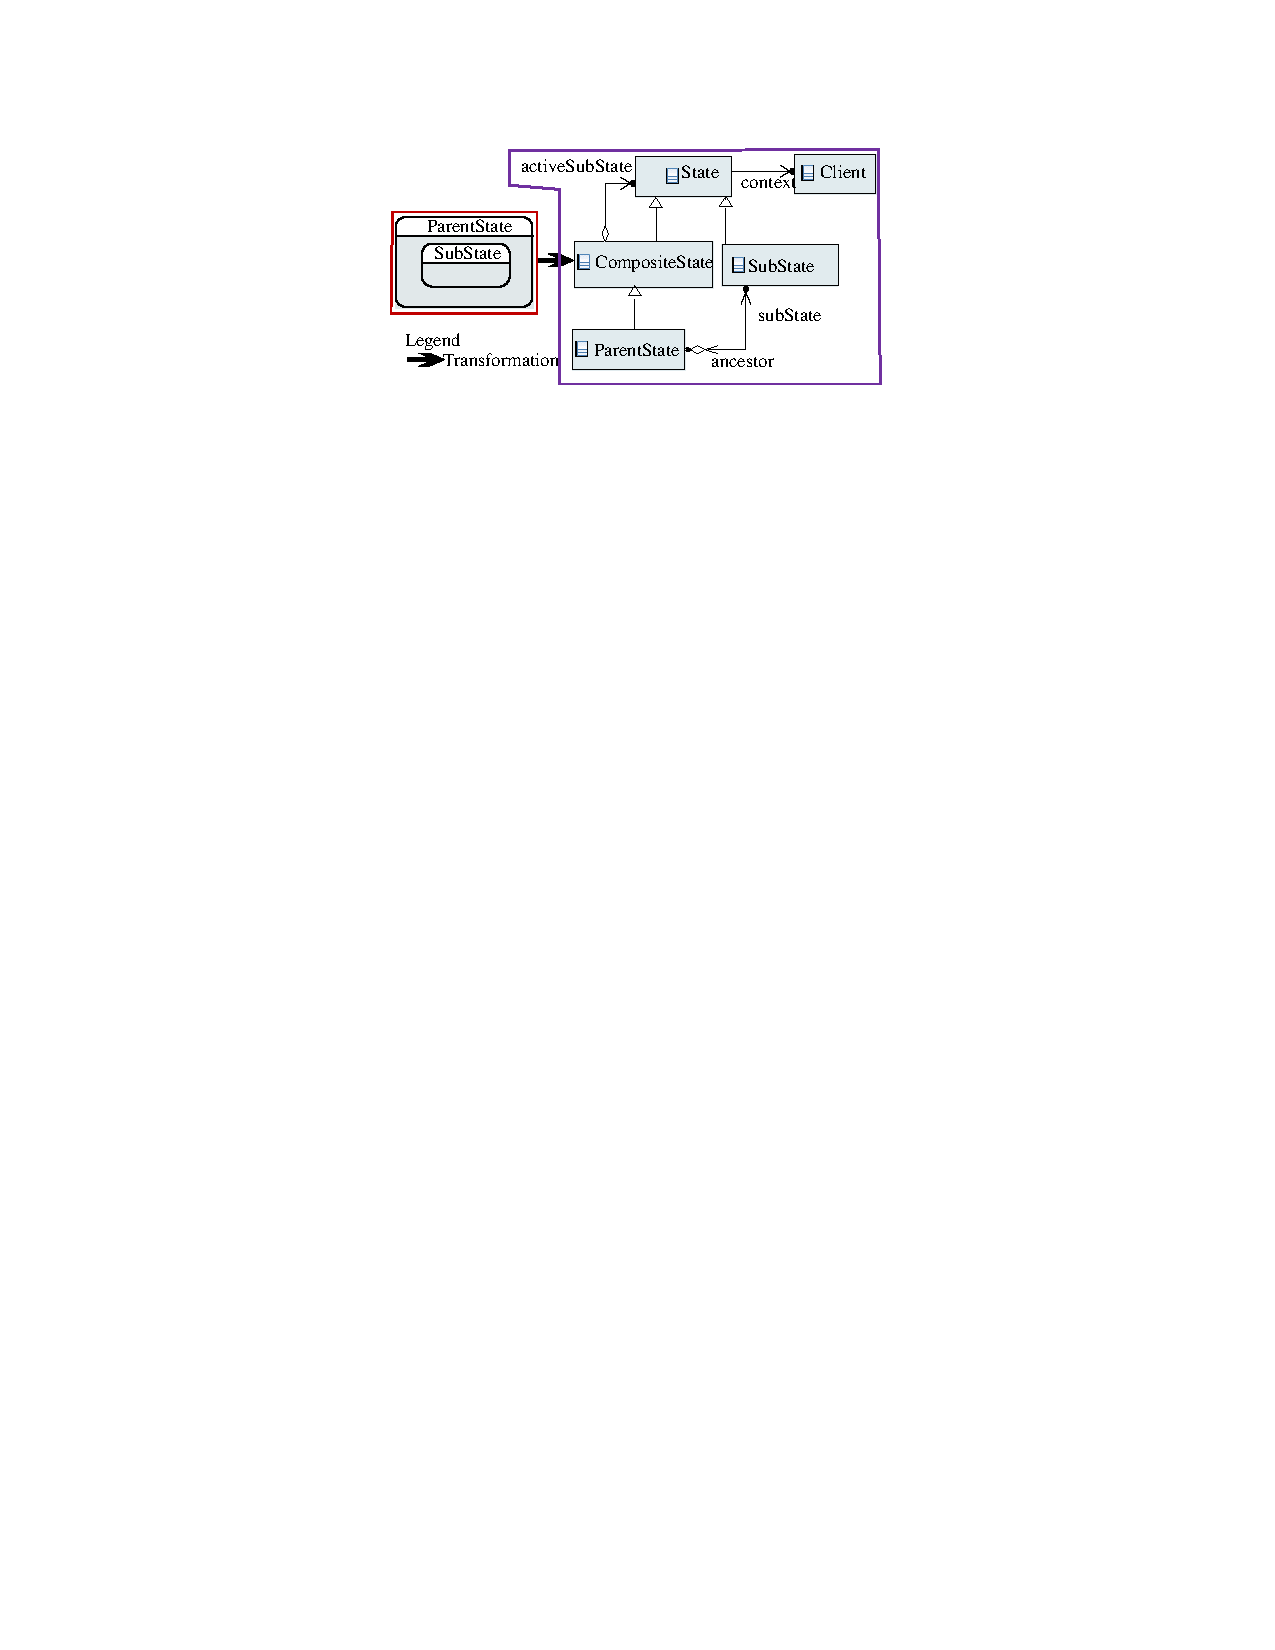
\includegraphics[clip, trim=6.5cm 21.3cm 0.5cm 2.4cm, width=0.8\textwidth]{figures/compositepattern}
\caption{Transformation from hierarchical state to class diagram} 
\label{fig:hierarchical-class}
\end{figure}

\subsubsection{Transformation of events}
\label{subsec:events}
DD has no means to convey data of events in the SM and considers every event as the same. In our approach, each event is transformed into a UML class that can contain data. Three different event class types corresponding to the UML event types \ti{CallEvent}, \ti{SignalEvent} and \ti{TimeEvent} are differentiated. An event class associated with a \ti{CallEvent} inherits from the base event class and contains the parameters in form of attributes typed by the same types as those of the operation associated with the \ti{CallEvent}. The operation must be a member of the provided interface of a port of the context class (a component as described above). For example, a call event \ti{CallEventSend} associated with an operation named Send, which has two input parameters typed by Integer, is transformed into a class \ti{CallEventSend} having two attributes typed by \ti{Integer}. When a component receives an event, the event object is stored in an event queue.

A signal event enters the component through a port typed by the signal. From the implementation view, this signal is transferred to the component by an operation provided by the component at the associated port. Therefore, the transfer of a signal event becomes similar to that of \ti{CallEvent}. For example, a signal event containing a data \ti{SignalData} arrives at a port p of a component C. The transformation derives an interface \ti{SignalDataInterface} existing as the provided interface of p. \ti{SignalDataInterface} has only one operation \ti{pushSignalData} whose body will be generated to push the event to the event queue of the component. Therefore, the processing of a \ti{SignalEvent} is the same as that of a \ti{CallEvent}. In the following section, the paper only considers \ti{CallEvent} and \ti{TimeEvent}.

A \ti{TimeEvent} is considered as an internal event. The source state class of a transition triggered by a \ti{TimeEvent} executes a thread to check the expiration of the event duration as in \cite{Niaz2004} and puts the time event in the event queue of the component. 

\subsubsection{Transformation of transitions and actions}
\label{subsec:transitions}
In this paper, actions and transition guards in the SM are considered as an operation associated with a block of code describing the actions behavior. Each action is transformed into an operation in the transformed context class. \ti{Entry/Exit/doActivity} actions have no parameters while transition actions and guards accepting the triggering event object have access to the event data. A transition is transformed into an operation taking as input the source state object and the event object similarly to DD. Transitions transformed from triggerless transition which has no triggering events accept only the source state object as a parameter.

Four ways of entering a composite state are differentiated. Three of these including a transition ending (1) on the border, (2) on a sub-state or (3) on a history state of a composite state are detailed in \cite{spinke_object-oriented_2013}. In the last one, a transition \ti{$t_{ex}$} ends (4) on an entry point of a composite state. Exact one transition \ti{$t_{in}$} allowed from an entry point ends on a sub-state of a composite state. Semantically, (4) is similar to (2) since both have the same sequential operations: executing the entry action of the composite state, execute the effect of \ti{$t_{in}$} in (4) or the transition \ti{$t_{default}$} from an initial pseudo state to the sub-state in (2). The transition \ti{$t_{in}$} is not allowed to have a guard or a trigger event similarly to the semantics of \ti{$t_{default}$}. 

Exiting a composite state is executed through exit points inversely to entry points. Each exit point has exactly one external corresponding outgoing transition representing a continuation of terminating incoming transitions.

In our implementation presented in Section \ref{sec:implementation} entry points and exit points are supported in both directions of the RTTRIP. 

\subsubsection{Storage of tracing information}
\label{subsec:trace}
The tracing information generated in the transformation is contained in a table. Mappings from UML SM concepts to UML classes are mainly one-to-one except for attributes referring composite state or sub-state. The table therefore only keeps identifiers as qualified names and types of elements in the SM model and the associated elements in the UML class model. The tracing table for the SM example in Figure \ref{fig:statemachuine} is shown in Table \ref{table:trace}.

In Figure \ref{fig:statemachuine}, the SM is contained in, for instance, the \ti{Client} component, \ti{Root} is the name of the source model. States of the SM are contained in a region \ti{TopRegion}. In the intermediate model, a package named \ti{PerClass\_Client} is created to contain all of transformed classes including ones associated with events and states. This package eases the maintenance of source code as well as the backward transformation of the RTRIP. The transition \ti{fromStoppedToOperating} is transformed into an operation transition inside the SM class which contains \ti{Stopped}. \ti{Initialize}, \ti{Enable}, \ti{Prepare}, and \ti{Disable} are transformed into operations in the context class \ti{Client}. It is worth noting that there can be several transitions outgoing from a state. Therefore, more than one transition in SM can be mapped to the same qualified name in the tracing table. In order to differentiate different transitions in the intermediate model, the qualified name of a transition operation in the intermediate model is combined with the source state and the triggering event. From this tracing table, it is easy to look back the original SM elements from the elements in the intermediate model in the backward direction. This transformation can be implemented as an in-place transformation but it would surprise users. Furthermore, the intermediate model should be used only as a bridge to the code and hidden to users. 

\begin{figure}
\centering
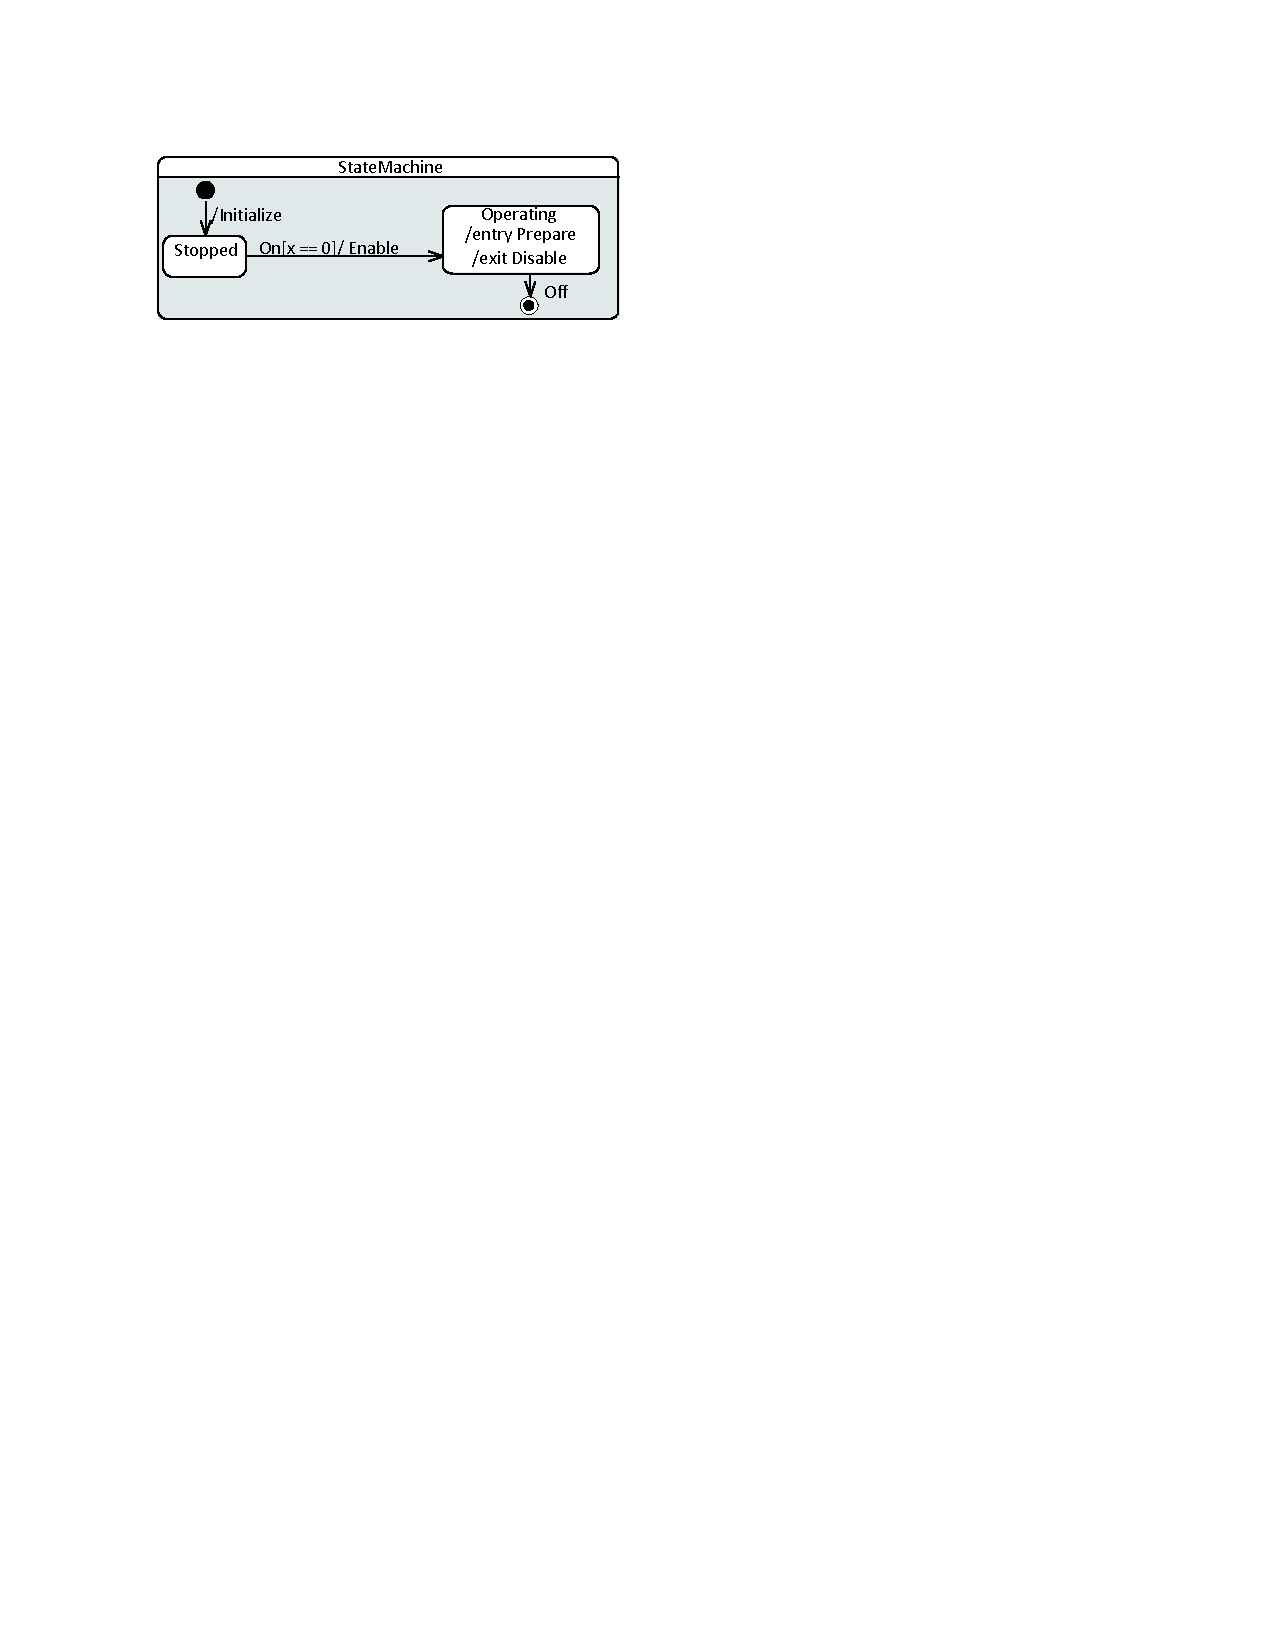
\includegraphics[clip, trim=2.5cm 22.5cm 10.5cm 2.5cm, width=0.4\textwidth]{figures/statemachine}
\caption{An example of SM for tracing table} 
\label{fig:statemachuine}
\end{figure}

\begin{table*}[]
\centering
\caption{Tracing table of state machine and class intermediate model}
\label{table:trace}
\begin{tabular}{|l|l|}
\hline
UML state machine concepts                                                 & UML class concepts                                     \\ \hline
Root::Client::StateMachine::TopRegion::Stopped (State)                     & Root::Client (Class)                                   \\ \hline
Root::Client::StateMachine (StateMachine)                                  & Root::Client::PerClass\_Client::StateMachine (Class)   \\ \hline
Root::Client::StateMachine::TopRegion::Stopped (State)                     & Root::Client::PerClass\_Client::Stopped (Class)        \\ \hline
Root::Client::StateMachine::TopRegion::Operating (State)                   & Root::Client::PerClass\_Client::Operating (Class)      \\ \hline
Root::Client::StateMachine::TopRegion::On (CallEvent)                      & Root::Client::PerClass\_Client::On (Class)             \\ \hline
Root::Client::StateMachine::TopRegion::Initialize(OpaqueBehavior)          & Root::Client::PerClass\_Client::Initialize (Operation) \\ \hline
Root::Client::StateMachine::TopRegion::Enable (OpaqueBehavior)             & Root::Client::PerClass\_Client::Enable (Operation)     \\ \hline
\end{tabular}
\end{table*}


The intermediate model is then used as input of a template-based object-oriented code generator. The use of an intermediate model facilitates the transformation from the SM to code and vice versa. Furthermore, the code generation process can use existing generators. Mappings from UML classes to object-oriented are trivial one-1-one. Listing \ref{lst:code-segment} shows a code segment generated from the SM in Figure \ref{fig:statemachuine}. The \ti{dispatchEvent} method implemented in the base composite state delegates an incoming event processing to its active sub-state. If the event is not accepted by the active sub-state, the composite state processes it. \ti{OnEntryAction} and \ti{OnExitAction} overwrite abstract methods which are defined in the base state class and called by the entry and exit methods, respectively. \ti{Stopped} accepts an \ti{On} event by implementing a corresponding \ti{processEvent} method. The transition method from the \ti{Stopped} to the \ti{Operating} state checks the guard condition by calling an associated method in the context class, then executes the transition action, changes the active state and finally enters the target state by calling entry. The machine enters the final state by setting the active state to null meaning that the behavior of the region containing the final state has completed. The generated code statements are intuitively similar to the UML SM semantics and it is easy to modify the behavior of the SM by code. For example, if we would like to change the default state, we only need to modify the \ti{setInitDefaultState} method by assigning the attribute \ti{activeSubState} to the attribute \ti{operating} that represent an instance of the state \ti{Operating}.

\subsubsection{Code generation}
\label{subsec:codegen}
\begin{minipage}{\linewidth}
\begin{lstlisting}[caption=A segment of C++ generated code, label=lst:code-segment]
class CompositeState: public State {
protected:
  State* activeSubState;
public:
bool dispatchEvent(Event* event) {
 if (activeSubState==NULL) {
  setIniDefaultState();
 }
 return activeSubState->
 dispatchEvent(event)||
this->processEvent(event);            
}}
StateMachine::StateMachine(Client* ctx){
  this->context = ctx;
  stopped = new Stopped(this, ctx);
  operating = new Operating(this, ctx);}
void StateMachine::setIniDefaultState(){
  this->context->Initialize();
  this->activeSubState = stopped;
  this->activeSubState->entry();}
bool StateMachine::transition(
        Stopped* state, On* event) {
 if(this->context->guard(event)){
  this->activeSubState->exit();
  this->context->Enable(event);
  this->activeSubState = this->operating;
  this->activeSubState->entry();
  return true;}
return false;}
bool StateMachine::transition(
    Operating* state, Off* event) {
  this->activeSubState->exit();
  //no action defined
  this->activeSubState = NULL;
return true;}
class Stopped: public State {
private:
  StateMachine* ancestor;
public: 
virtual bool processEvent(On* event) {
  return this->ancestor->transition(this,event);}
}
\end{lstlisting}
\end{minipage}

\subsection{Merging from modified code to UML SM}
This section describes the backward process. 

\subsubsection{Method Overall}
The generated code can be modified by adding/removing/changing states, transitions, actions. The modified generated code then needs to be reversed back to the SM to make the artifacts consistent. The overall method for backward transformation is shown in Figure \ref{fig:details}. The modified code is first verified by partly inspecting the code syntax and semantics to guarantee that the semantics of SM in the code is correct. This step is needed since not all of code modifications can be reversed back to the SM. The verification also produces an output (\ti{output2}) whose format is described later. If the intermediate model or the original SM is absent, a new intermediate model and a new SM are created. In the contrary, the intermediate model is used for generating the previous version of code or the previous code can be taken from control versioning systems. The previous code is also verified to have its output (\ti{output1}). \ti{Output1} and \ti{Output2} are then compared with each other to detect actual semantic changes which are about to be propagated to the original model. 

\begin{figure}
\centering
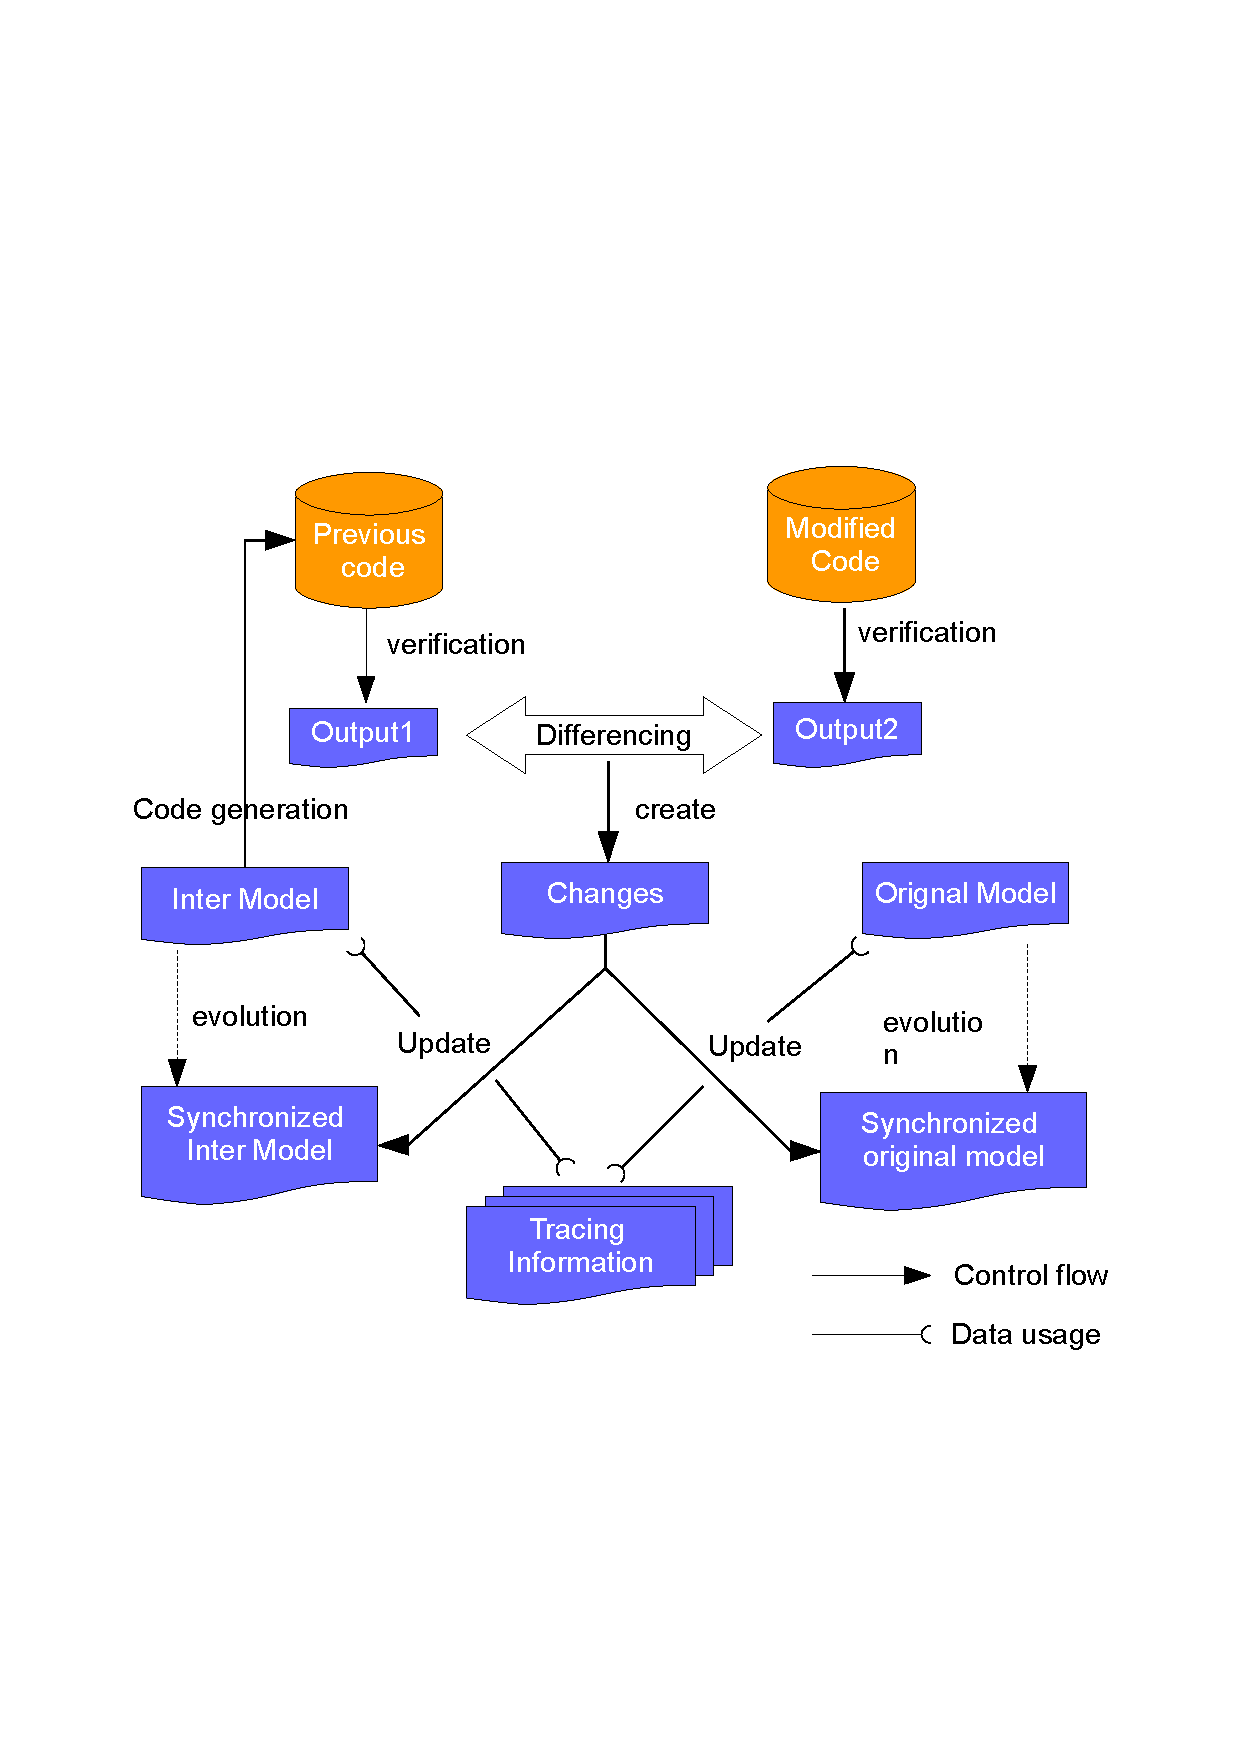
\includegraphics[clip, trim=1cm 7cm 0.1cm 7.8cm, width=0.47\textwidth]{figures/details.pdf}
\caption{Overall method for reversing code to state machine} 
\label{fig:details}
\end{figure}

\subsubsection{Semantic Verification}
The information contained by the output of the semantic verification is a list of event names, a list of state names, a list of transitions in which each has a source state, a target state, a guard function, an action function and an event represented in so called abstract syntax tree (AST) transition [15]. For example, Figure \ref{fig:transitions} presents the EMF \cite{gronback_eclipse_} representation of transitions in \tb{C++} AST in which \ti{IStructure} and \ti{IFunctionDeclaration} represent a structure and a function in \tb{C++}, respectively. Each state name is also associated with an ancestor state, an entry action, an exit action, a default sub-state and a final state. The output is taken by analyzing the AST. The verification process consists of recognizing different patterns. The pattern list is as followings:

\tb{State}: A state class inherits from the base state class or the composite base state class. For each state class, there must exist exactly one attribute typed by the state class inside another state class. The latter is the ancestor of the state class.

\tb{Composite state}: A composite state class (CSC) inherits from the base composite state. For each sub-state the CSC has an attribute typed by the associated sub-state class. The CSC also implements a method named \ti{setInitDefaultState} to set its default state. The CSC has a constructor is used for initializing all of its sub-state attributes at initializing time.

\ti{Entry action}: If a state has an entry action, its associated state class implements \ti{onEntryAction} that calls the corresponding action method implemented in the context class. If the state has outgoing \ti{triggerless} transitions, \ti{onEntryAction} appeals the \ti{triggerless} transition method of the ancestor state class following the entry action call.

\tb{Exit action}: Similar to the entry action pattern but implements \ti{onExitAction}.

\tb{Event processing}: If a state has an outgoing transition triggered by an event, the state class associated with the state implements the \ti{processEvent} method having only one parameter typed by the event class transformed from the event. The body calls the corresponding transition method of the ancestor class.
\ti{CallEvent} class: A call event class inherits from the base event class. The call event class contains attributes typed by the parameter types of the operation associated with the call event. This pattern is detected if the types of attributes of the event class match with the types of parameters of one of the methods in the context class. There is therefore an ambiguity for an event class to choose an associated operation if more than one operation detected matches the event class. Hence, this pattern poses a restriction that operations associated with events must either have different parameter types or different number of parameters. To overcome this issues, a naming convention used for \ti{CallEvent} classes is used. The event class name is prefixed with the associated operation name. If the event class name does not follow the naming convention, the reverse is refused. Another possible solution targeting this ambiguity is to have a user interaction in case of having more than one operation matching with the event. Having an interaction allows the pattern detection get rid of ambiguity and therefore provides appropriate SM models. A signal event is treated as a \ti{CallEvent} as previously described.

\tb{Time event}: A transition is triggered by a \ti{TimeEvent} if the state class associated with its source state implements the timed interface. The duration of the time event is detected in the transition method whose name is formulated as \ti{"transition" + duration}. 

\tb{Transition}: Transition methods are implemented in the ancestor class of the source state class. Two types of transition methods correspond to trigger and \ti{triggerless} transitions. Both \ti{parameterize} its source state class. The trigger transition method has an additional parameter typed by the event class associated with the event triggering the transition. The body of transition methods contains ordered statements including exiting the active state, executing transition action (effect), changing the active state to the target or null if the target is the final state, and entering the changed active state by calling entry. The body can have an if statement to check the guard of the transition. The transition action and the guard are optional. Several if/else statements can appear in a \ti{triggerless} transition method body.

\tb{Transition action/guard}: Transition actions and guards are implemented in the context class.

\begin{algorithm}[H]
  \caption{Semantic verification
    \label{alg:semantic-vefrification}}
  \begin{algorithmic}[1]
    \Require{AST of code and a list of state classes stateList}
	\Ensure{Output of semantic verification}
    %\Statex
    	\For {$s$ in $stateList$}
        	\For {$a$ in attribute list of $s$}
        		\If {$a$ and $s$ match child parent pattern}
        			put a and s into a state-to-ancestor map;
        		\EndIf
        	\EndFor
        	\For {$o$ in method list of $s$}
        		\If {$o$ is $onEntryAction$ || $o$ is $onExitAction$}		\State $verifyEntryExit(o)$; 	
        		\ElsIf {$o$ is $processEvent$} 
        			\State $verifyProcessEvent(o)$;
        		\ElsIf {$o$ is $setInitDefaultState$ \& $s$ is composite}
        			\State $verifyInitDefaultState(s)$;
        		\ElsIf {$o$ is timeout \& $s$ is a timedstate}
        			\State $verifyTimeoutMethod(o)$;
        			\State $verifyProcessEvent(s,o)$;
        		\EndIf	
        	\EndFor
    	\EndFor
  \end{algorithmic}
\end{algorithm}

Listing \ref{alg:semantic-vefrification} shows the algorithm used for verifying code semantics. Because of limited space, \ti{verifyEntryExit}, \ti{verifyProcessEvent}, \ti{verifyInitDefaultState}, \ti{verifyTimeoutMethod} and \ti{verifyProcessEvent} are not presented but they basically follow the pattern description as above. In the first step of the verification process, for each state class, it looks for an attribute typed by the state class, the class containing the attribute then becomes the ancestor class of the state class. The third steps checks whether the state class has an entry or exit action by looking for the implementation of the \ti{onEntryAction} or \ti{onExitAction}, respectively, in the state class to recognize the \ti{Entry/Exit} action pattern. Consequently, event processing, initial default state of composite state and time event patterns are detected following the description as above.  Figure \ref{fig:partition} shows the partitioning used for matching code segments to SM elements. Each partition consists of a code segment and the corresponding model element which are mapped in the backward direction. For instance, the \ti{Stopped} class in code is detected as a representation since it inherits from the base class \ti{State}.  
 
\begin{comment}
\begin{figure}
\centering
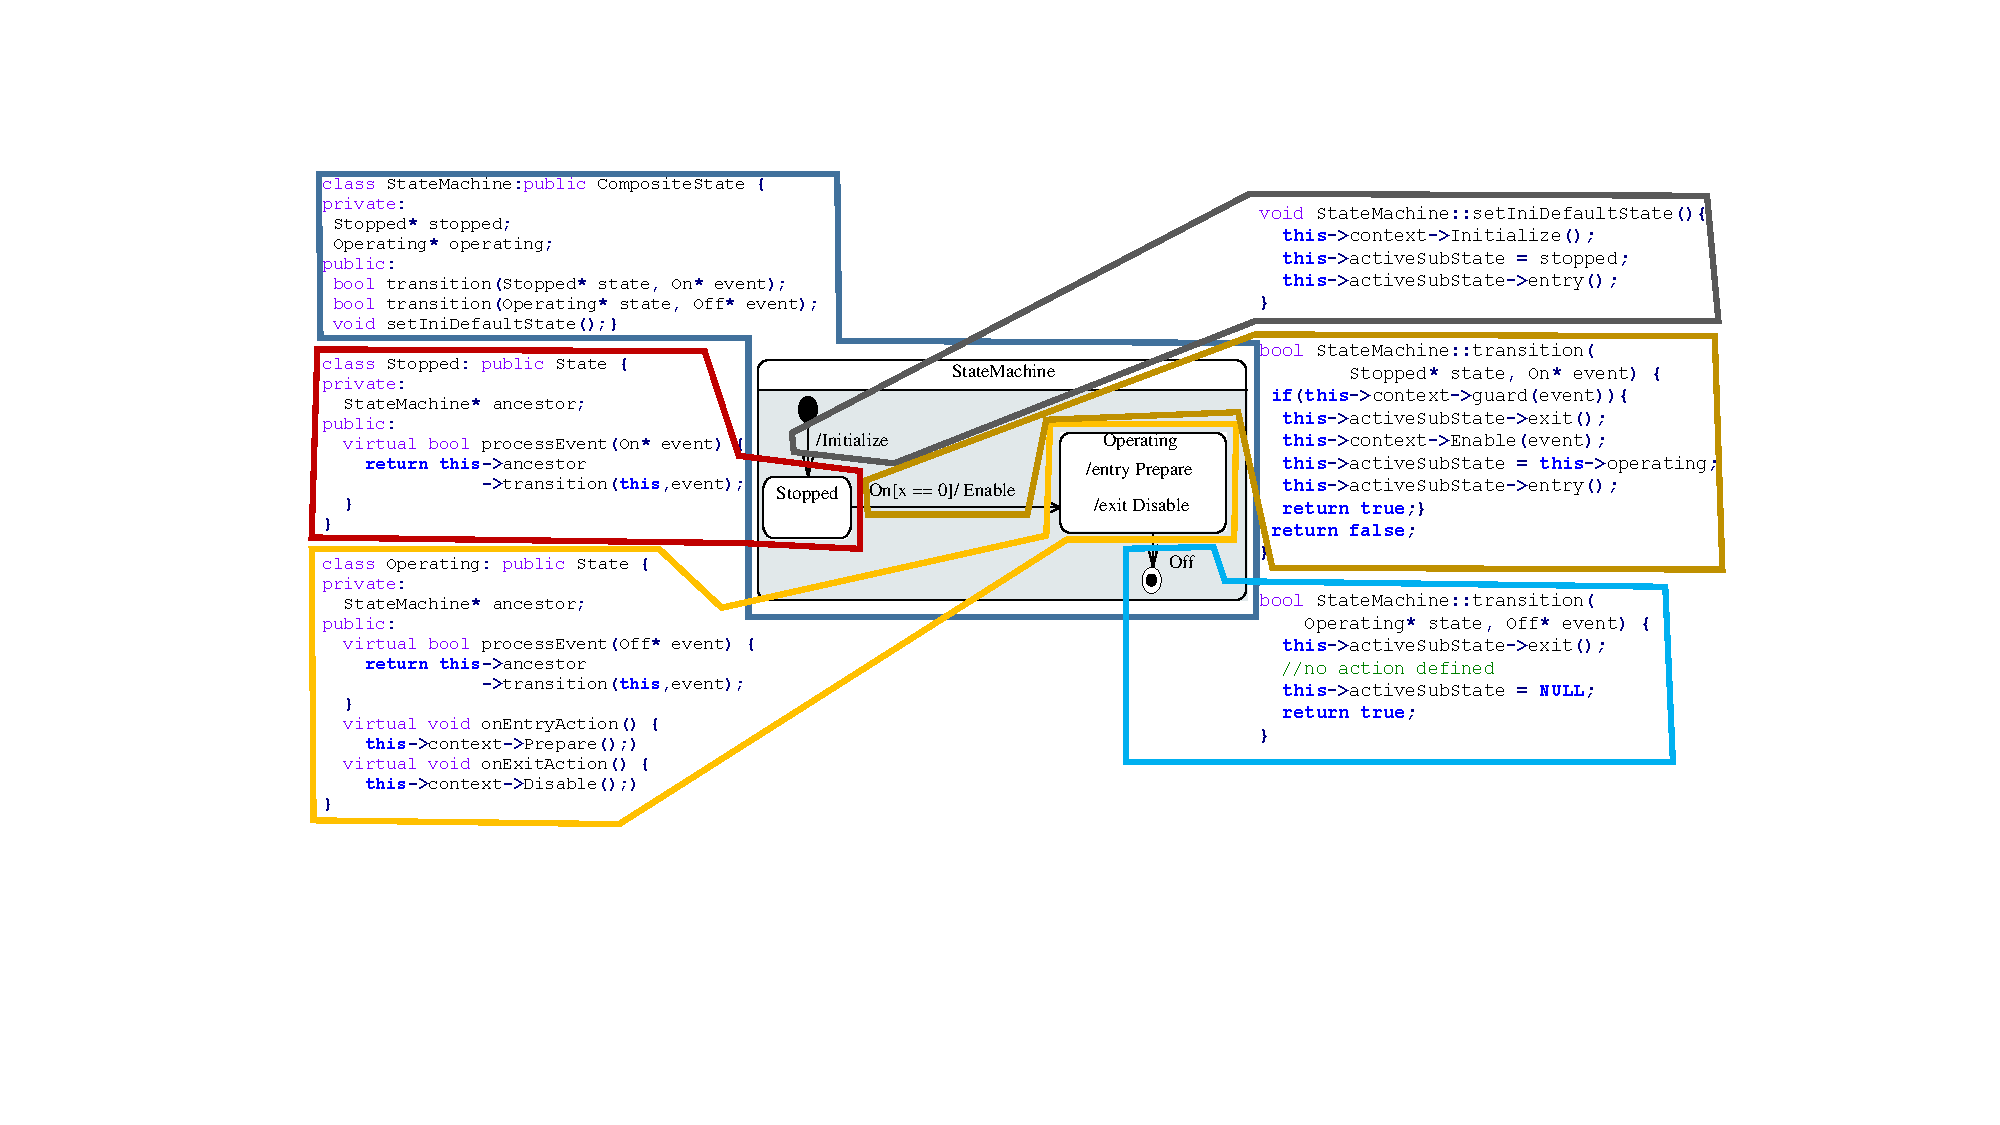
\includegraphics[clip, trim=1cm 4.8cm 0.1cm 0.8cm, width=0.75\textwidth]{figures/backwardmapping.pdf}
\caption{SM element-code segment mapping partition} 
\label{fig:partition}
\end{figure}
\end{comment}

\begin{figure}
\centering
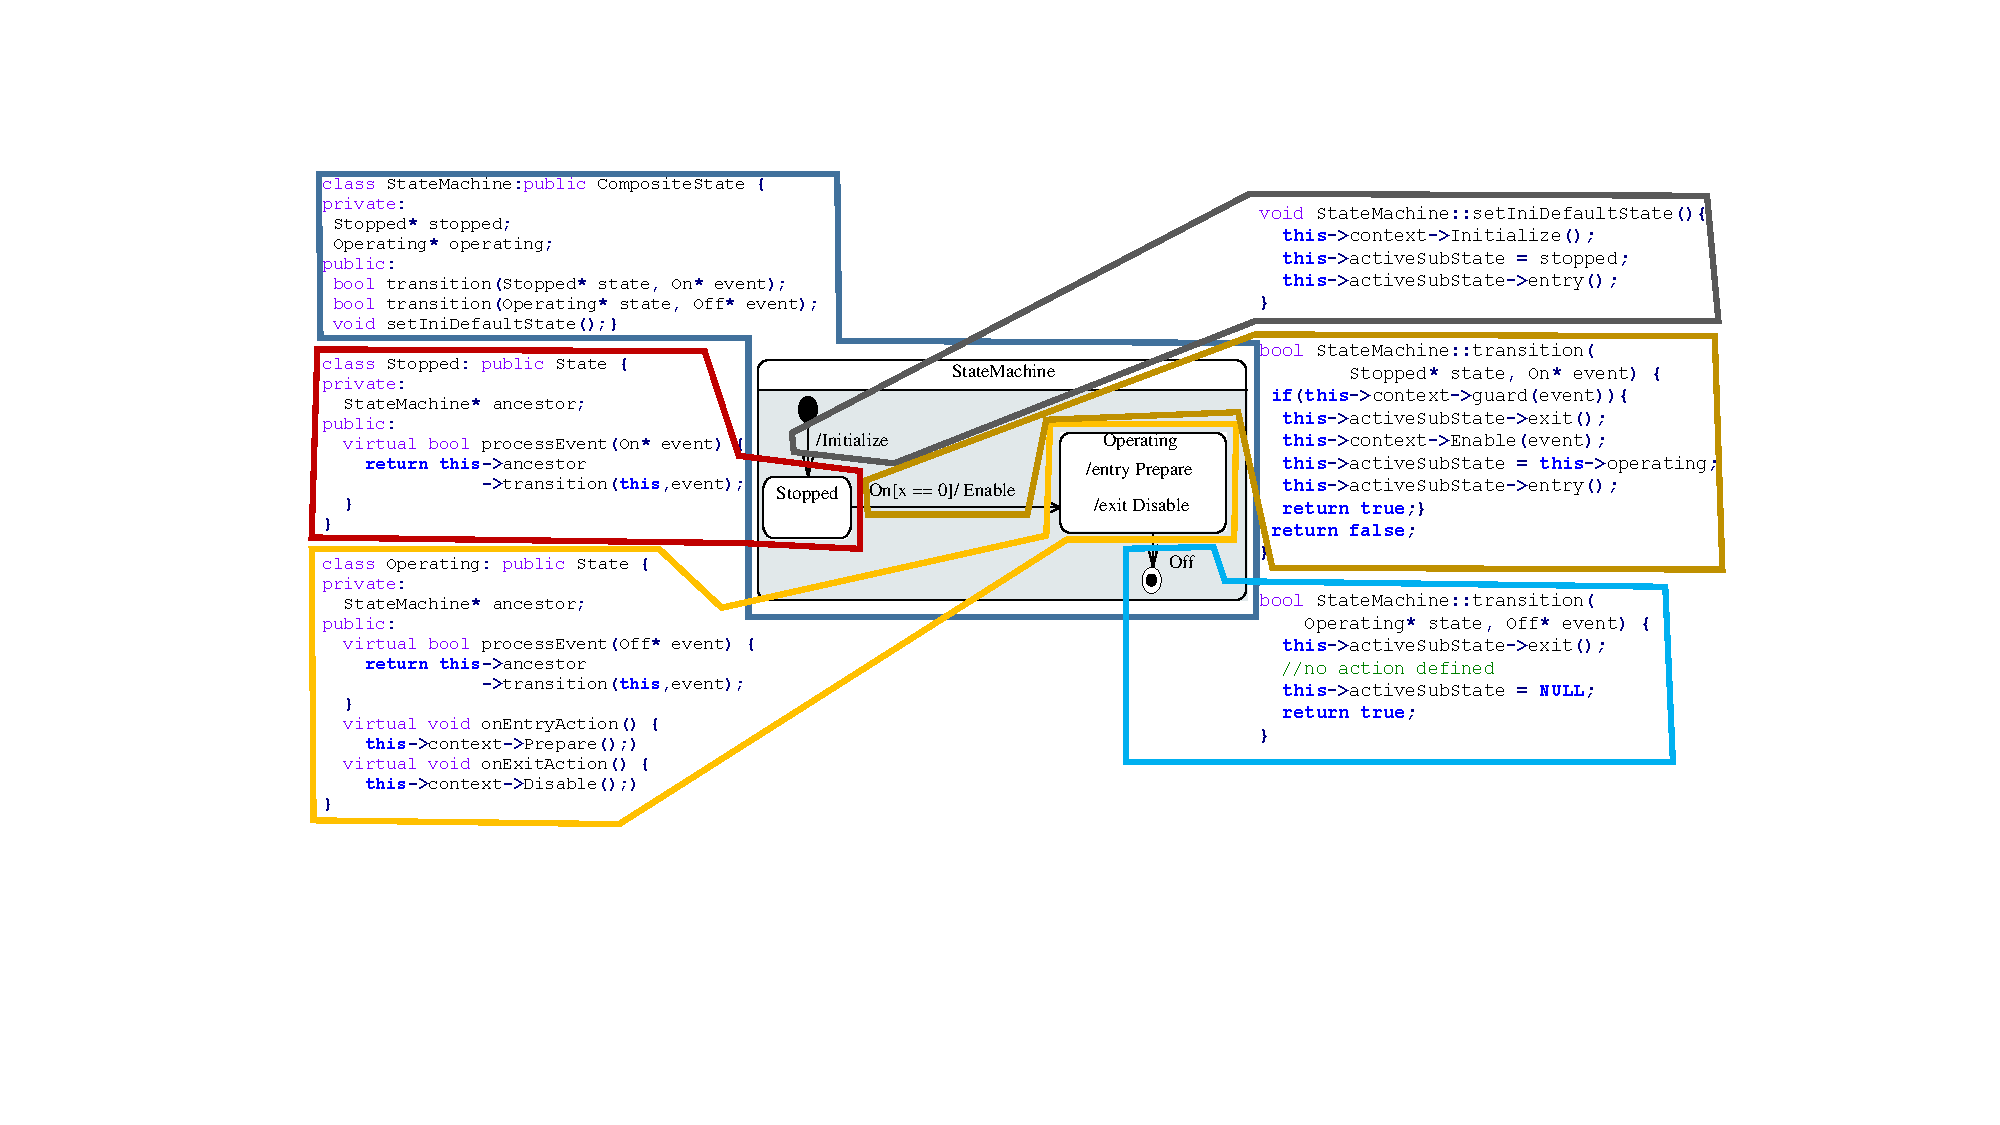
\includegraphics[clip, trim=5.2cm 5.1cm 0.1cm 2.8cm, width=0.52\textwidth]{figures/backwardmapping.pdf}
\caption{SM element-code segment mapping partition} 
\label{fig:partition}
\end{figure}

\begin{figure}
\centering
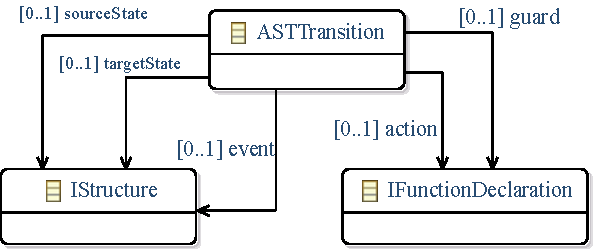
\includegraphics[clip, trim=0cm 0.06cm 0.0cm 0.08cm, width=0.3\textwidth]{figures/asttransition}
\caption{Transitions output from the verification of code} 
\label{fig:transitions}
\end{figure}

\subsubsection{Construction of SM from verification output}
If an intermediate model is not present, a new intermediate model and a new SM are created by a reverse engineering and transforming from the output of the verification process. The construction is straightforward. At first, states are created. Secondly, UML transitions are built from the AST transition list. Action/guard/triggering event of a UML transition is created if the associated AST transition has these.

\subsubsection{Updating the original SM from modified code}
In contrast to the previous sub-section, if an intermediate model is existing, it is also transformed into lists of states and transitions. The output of verification process and that of intermediate model transformation are compared to each other to detect the semantics changes of the modified code. The algorithm for detecting state and transition changes is shown in Listing \ref{alg:semantic-vefrification}.

The algorithm takes as input lists of state names, transitions, ancestor maps extracted from the intermediate model and the modified code, respectively. The algorithm results in lists of state names, transitions to be added/deleted/updated/moved. It first examines the list of state names extracted from the modified code $Lc$ for states that are not existing in the list of state names of the intermediate model $Li$ to be added to the added state list. If a state $c$ in $Lc$ is present in $Li$, $c$ is either added to the updated list if the ancestor states associated with $c$ in the intermediate model and the modified code are the same, or $c$ is considered as being moved to another ancestor state. Other states in $Li$ are added to the deleted state list. The transition change detection is similar to that of states but instead of checking by name, the source and target state names of transitions and the associated event name in $Tc$ and $Ti$ are used. Together with states and transitions but not presented in Listing \ref{alg:change-detect}, event changes are also detected similarly.

The changes detected by the algorithm are then used in a change propagation step which updates the original SM. Events, states and transitions are sequentially processed in order. The processing of deleted elements results in deleting corresponding elements in the SM. A deleted element in code is associated with an element in the intermediate model. As previously described, the mapping information for elements in code and the intermediate model is also stored in a table. Therefore, it is trivial to retrieve the model element in the intermediate model associated with the deleted element.

The found model element in turn helps identify the associated element in the SM by using the mapping table between the SM and the class model. For each deleted event in code, the associated event class in the class model and the event in the SM are deleted. Deleted states and transitions are similarly propagated. A deletion of a transition includes deleting its guard, triggers and transaction action. 
\begin{algorithm}[H]
  \caption{Change detection
    \label{alg:change-detect}}
  \begin{algorithmic}[1]
    \Require{$Li$, $Lc$, $Ti$, $Tc$, $mapI$, $mapC$ are lists of state names, transitions, ancestor map extracted from intermediate model and modified code, respectively}
	\Ensure{$adS$, $delS$, $uptS$, $movS$ are lists of added, deleted, updated and moved states respectively. $adT$, $delT$, $uptT$ are lists of added, deleted and updated transitions}
    %\Statex
    	\For {$c$ in $Lc$}
        	\If {!$Li$.contains($c$)} 
				\State adS.put(c);
        	\Else
				\If {$mapC$.get($c$) = $mapI$.get($c$)}
	    			\State uptS.put(c);
				\Else 
	    			\State $movS$.put($c$, $mapI$.get($c$), $mapC$.get($c$))	
                \EndIf
                	\State $Li$.remove($c$);
        	\EndIf
    	\EndFor
    	\For {$i$ in $Li$} 
        	\State $delS$.put($i$)
    	\EndFor
    	\For {$c$ in $Tc$}
        	\State $found$ = NULL
        	\For {$i$ in $Ti$}
				\If {$c$.source=$i$.source \& $c$.target=$i$.target \& $c$.event = $i$.event}
	    			\State $found$ = $i$;
              	\EndIf
             \EndFor 	
        	\If {$found$ != NULL} 
				\State $uptT$.put($c$);
				\State $Ti$.remove($found$);
        	\Else
				\State $adT$.put($c$);
        	\EndIf
    	\EndFor
    	\For {$t$ in $Ti$}
        	\State $delT$.put($t$);
    	\EndFor
  \end{algorithmic}
\end{algorithm} 
For each added event in code, an event is added to the class model and in turn to the SM. For each added state, its ancestor state is retrieved through the mapping tables, a new state is then created and attached to the ancestor. Entry and exit actions are also added to the new state afterward. A moved state is handled by looking for the associated state, the old and new ancestor state in the SM, and moving the associated state to the new ancestor. Each added transition is propagated by creating a new transition in the SM and retrieving source and target states from the mapping tables. An update is executed by looking in the mapping tables for elements in the SM associated with elements updated in code. It is worth noting that this algorithm detects a renaming of an event or state as a deletion followed by an addition. 


  
For example, assuming that we need to adjust the SM example shown in Figure \ref{fig:statemachuine}  by adding a guard to the transition from \ti{Operating} to the final state. The adjustment can be ordered by either modifying the SM model or the generated code. In case of code, the associated transition function in Listing \ref{lst:code-segment} is edited by inserting an if statement which calls the guard method implemented in the context class. The transition function becomes as in Li. The algorithm in Listing \ref{alg:change-detect} adds the transition function into the updated list since it finds that the source state, the target state and the event name of the transition is not changed. By using mapping information in the mapping table, the original transition in the SM is retrieved. The guard of the original transition is eventually created. 	





